\documentclass[11pt,a4paper]{article}
\usepackage[utf8]{inputenc}
\usepackage[german]{babel}
\usepackage{amsmath}
\usepackage{amsfonts}
\usepackage{subfig}
\usepackage{amssymb}
\usepackage{siunitx,physics}
\usepackage{mathtools}
\usepackage{graphicx}
%\usepackage{Here}
\usepackage[version=4]{mhchem}
\usepackage{url}
\usepackage{setspace}
\usepackage[left=2.5cm,right=2.5cm,top=2.5cm,bottom=2cm]{geometry}
[biblography=totocnumbered]
\usepackage{fancyhdr}
\usepackage{scrextend}
\usepackage{hyperref}
\pagenumbering{gobble}

\makeatletter
\newcommand\bigcdot{\mathpalette\bigcdot@{.5}}
\newcommand\bigcdot@[2]{\mathbin{\vcenter{\hbox{\scalebox{#2}{$\m@th#1\bullet$}}}}}
\makeatother

\makeatletter
%\renewcommand*\bib@heading{%
%  \subsection*{}%
%  \@mkboth{\refname}{\refname}}
%\makeatother
\numberwithin{equation}{section}
\numberwithin{figure}{section}

\renewcommand{\labelitemii}{\labelitemfont$\vartriangleright$}
\begin{document}\\
\begin{addmargin}[25pt]{0pt}
In Abbildung \ref{fig:Enthalpie_Phasenumwandlung} sind der Oberflächenanteil (rot), der Volumenanteil (blau) und die Gesamtenthalpieänderung (grün) gegen den Radius geplottet. Man erkennt, dass ab einem kritischen Radius $r^*$ die Keime stabil sind und weiter wachsen, bei niedrigeren Radien lösen sie sich wieder auf. Aus der Bedingung $\frac{\si{d} \Delta G}{\si{d}r} = 0$ am Ort des kritischen Radius findet man:
\begin{align}\label{eq:kritischer_Radius}
    r^* &=-\frac{2\gamma}{\Delta G_V}\\\label{eq:Aktivierungsenergie}
    \Delta G^* &= \frac{16\pi\gamma^3}{3(\Delta G_V)^2}
\end{align}
\begin{figure}[h]
    \centering
    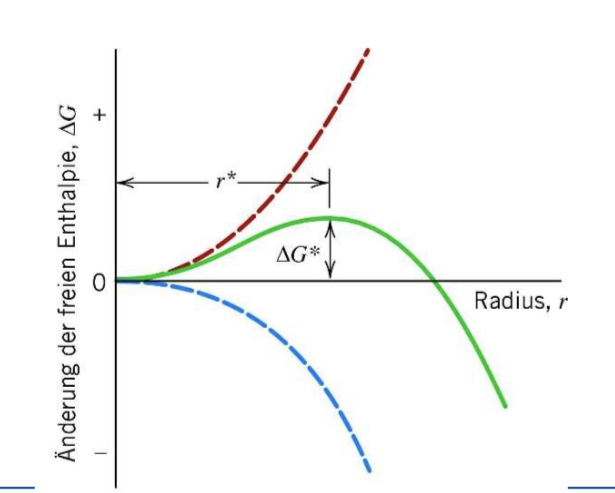
\includegraphics[width = 0.8\textwidth]{images/Materialwissenschaften/Enthalpie_Phasneumwandlung.jpeg}
    \caption{In rot ist der Oberflächenanteil, in blau der Volumenanteil und in grün die gesamte Änderung der Enthalpieänderung eines Keims zu sehen, der kritische Radius $r^*$ und die Aktivierungsenergie $\Delta G^*$ sind ein Maß dafür ab welchen Bedingungen die Keime weiter wachsen und sich nicth wieder auflösen}
    \label{fig:Enthalpie_Phasenumwandlung}
\end{figure}
\end{addmargin}

\end{document}